\chapter{Metodologia de pesquisa}\label{cap:metodologia}

Este estudo adotou uma abordagem qualitativa e de natureza exploratória, 
utilizando principalmente métodos de pesquisa bibliográfica para investigar o método ABA. 
Nesta seção, são delineados os detalhes fundamentais da metodologia empregada, 
incluindo a escolha do tipo de pesquisa, as técnicas e instrumentos utilizados, 
assim como os métodos de coleta e análise de dados.

A pesquisa de natureza exploratória foi escolhida devido à sua abordagem independente de estudos prévios, 
o que possibilita uma análise detalhada e uma compreensão mais completa dos fenômenos em questão. 
A pesquisa bibliográfica desempenhou um papel crucial ao fornecer uma base sólida para compreender e 
contextualizar o atual estado de conhecimento sobre o tema \cite{casula2021potential}.

Os métodos de coleta de dados consistiram nos testes de entrada e saída e testes unitários de métodos e funções. 
Os testes foram feitos usando recursos e bibliotecas do próprio 
\textit{framework} que fornece os dados, mostrando o que cada entrada gera de saída. 
Posteriormente, os dados são avaliados através de uma análise, 
visando extrair informações pertinentes e estabelecer relações significativas dentro do contexto estudado.

Para complementar a coleta de dados, foram conduzidos testes de entrada e saída no \textit{software} desenvolvido. 
Esses testes serviram para avaliar a interação do usuário com a aplicação, 
verificando a resposta do sistema às entradas do usuário e garantindo a saída correta dos dados processados.

Os testes unitários foram implementados para as princimais métodos e funções do \textit{software}, 
assegurando a correta execução de cada componente de maneira independente \cite{neto2007introduccao}. 
A análise de custo envolveu a avaliação dos recursos computacionais necessários para o funcionamento adequado do sistema.

% A análise de usabilidade e acessibilidade, realizada após a coleta de dados, será fundamental para avaliar a facilidade de uso do software e sua adaptação para diferentes usuários. pretende-se que essa análise proporcione \textit{insights} sobre possíveis melhorias na interface e na interação do usuário com o sistema.

Para realizar os testes de usabilidade, serão escolhidos profissionais que, por sua vez, 
irão convidar uma família com filho autista para testar a interface. 
A análise de usabilidade e acessibilidade, realizada após a coleta de dados, 
será fundamental para avaliar a facilidade de uso do \textit{software} e sua adaptação para diferentes usuários. 
Pretende-se que essa análise proporcione insights sobre possíveis melhorias na interface e na interação 
do usuário com o sistema.

% fim correção 

Essa abordagem metodológica foi selecionada para manter o foco na eficiência do 
\textit{software}, garantindo uma experiência de usuário intuitiva e amigável. 
Além disso, essa metodologia proporciona uma forma diferenciada de análise de dados das sessões e de treino com os pacientes, 
contribuindo para um avanço na área terapêutica do autismo.

% ---
% Capitulo de Resultados
% ---

% \chapter{Resultados}\label{cap:resultados}

\section{Ferramentas de desenvolvimento}
Este estudo apresentou o desenvolvimento de uma aplicação móvel com suporte \textit{web}, 
o que exigiu a utilização de ferramentas e padrões de projeto adequados. 
A escolha da tecnologia adotada permitiu a compilação para \textit{Android} nativo e \textit{web}. 
Com base nesses requisitos, optou-se pela utilização do \textit{framework} Flutter com a linguagem Dart, 
que oferece essa flexibilidade com adaptações mínimas entre as diferentes plataformas.

A interface, baseada em Flutter Dart, utiliza recursos do material do \textit{framework}, 
simplificando o design sem exigir amplo conhecimento de design. 
O Flutter é conhecido por sua estrutura de \textit{widgets}, 
facilitando a criação de \textit{layouts} \cite{windmill2020flutter}.

Para o desenvolvimento da API, a escolha recai em um \textit{framework} eficiente, 
com vasto suporte online e agilidade no desenvolvimento. 
Diante disso, entre o uso de PHP Laravel, Node.js, Spring Boot e Quarkus Java, 
optamos pelo Quarkus Java devido à velocidade e à vasta documentação disponível na internet. 
Logo, o Quarkus se torna altamente eficiente na criação de APIs \cite{koleoso2020welcome}.

\section{Padrões de projeto}

Na requisição para a API é usado o padrão \textit{RESTful} 
para URIs mais padronizadas e métodos HTTP diferentes para cada tipo de ação \cite{rodriguez2008restful}. 
A comunicação ocorre via JSON e são utilizados objetos DTO \footnote{
    Objetos DTO (Data Transfer Object) são classes simples que transferem dados entre 
    subsistemas de um \textit{software}. São um padrão de projeto de \textit{software} que 
    encapsulam dados para que possam ser transferidos entre camadas de uma aplicação.
} para simplificar a transferência de dados.


\begin{figure}[h]
{}
    \centering
    \caption{Ilustração do \textit{Atomic Design}}
    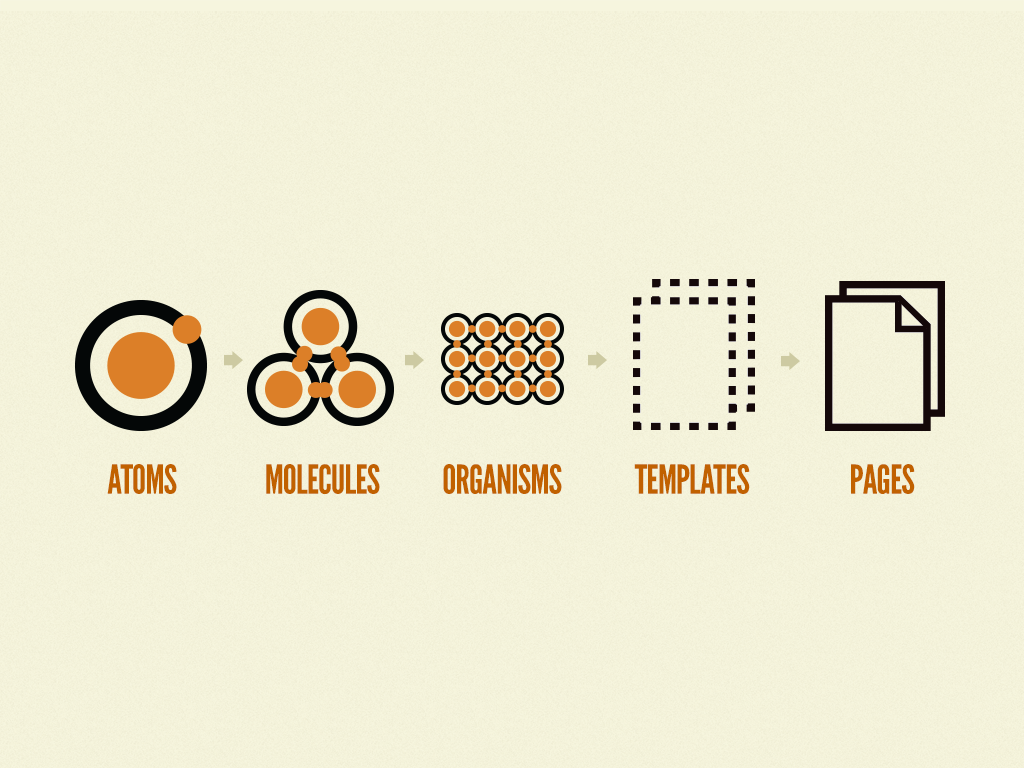
\includegraphics[scale=0.4]{imagens/Atomic_design.png} \\
    \label{fig:athomic_design}
    {
        % \bibitem{atomicDesign}
        FROST, Brad. \textit{Atomic Design}. 
        Disponível em: \url{https://bradfrost.com/wp-content/uploads/2013/06/atomic-design.png}. Acesso em: 02 dez. 2024.
    }
\end{figure}

\section{Levantamento de Requisitos}

O \textit{framework} utilizado na API adota injeção de dependência para facilitar a criação de funcionalidades 
e promover um desenvolvimento modular \cite{seemann2019dependency}. São empregados objetos específicos para a 
interação com o banco de dados: os \textit{Services} são responsáveis pela obtenção de dados, 
enquanto os \textit{Repositories} lidam com as alterações nos valores armazenados. 
No front-end, o desenvolvimento foi estruturado utilizando o conceito de \textit{Atomic Design}, 
que organiza os componentes em diferentes níveis: 
\textit{atoms}, \textit{molecules}, \textit{organisms}, \textit{templates}, e \textit{pages}. 
Os \textit{atoms} representam os menores elementos, enquanto as \textit{pages} são as páginas completas, 
formadas pela composição desses componentes \cite{frost2016atomic}, conforme ilustrado na Figura \ref{fig:athomic_design}.

\pagebreak

Com base na revisão da literatura apresentada na Seção \ref{cap:referencial_teorico}, 
identificou-se que o excesso de anotações em papel, comum na aplicação do método ABA, 
pode ser um obstáculo à eficiência do processo. As anotações, geralmente feitas por escrito, 
foram categorizadas em dois formatos para o sistema proposto: 
anotações em texto livre e anotações com opções predefinidas, 
como “acerto”, “erro” e “acerto com dica”. 
Essas opções podem ser personalizadas a qualquer momento, 
permitindo que o sistema seja flexível tanto para usuários com pouca familiaridade com tecnologias 
complexas quanto para aqueles que possuam maior experiência.

Os estímulos foram incorporados ao sistema de forma que o terapeuta possa apresentar um dispositivo 
(preferencialmente um \textit{tablet}, devido ao tamanho da tela, ou qualquer outro dispositivo móvel) ao paciente, 
que deverá interagir com o estímulo apresentado conforme o comando do terapeuta. 
As informações geradas durante essas sessões podem ser compartilhadas com a família do paciente, 
dependendo da configuração estabelecida pelo terapeuta.

Para garantir a participação ativa da família no desenvolvimento da criança, 
o sistema permite que eles acessem determinadas anotações realizadas pelo terapeuta. 
Além disso, caso a configuração de permissão de anotações esteja ativada, 
os familiares poderão fazer suas próprias observações. 
Em caso de desvinculação entre o terapeuta e o paciente, 
a família continuará tendo acesso a todas as anotações previamente realizadas pelo terapeuta.

\section{Funcionalidades do \textit{software}} 

O \textit{software} engloba dois perfis de usuários principais: 
terapeutas e famílias, cada um com seus privilégios e áreas específicas de acesso. 
As famílias têm acesso restrito somente às informações permitidas pelo terapeuta.

O perfil de terapeuta acessa dados compilados e formatados para oferecer uma visão geral dos pacientes, 
incluindo médias de levantamentos recentes. Além disso, 
o sistema oferece estatísticas sobre o número de pacientes em diferentes níveis e tipos de programa terapêutico.

O perfil de terapeuta também pode visualizar uma lista de pacientes, 
realizar ações básicas e acessar dados e anotações específicas de um paciente selecionado. 
Durante novos levantamentos de dados, o sistema solicita permissão das famílias para acessar informações específicas, 
além de permitir a definição do nível de dificuldade e programa terapêutico, quando necessário.

Durante os treinos, o sistema exibe um conjunto de cartões para o paciente, 
incluindo o cartão que representa o cenário de sucesso. 
Cada interação do paciente com o aplicativo é registrada instantaneamente, 
e os dados são enviados ao servidor para consulta futura. 
A sequência das ações realizadas pelo \textit{software} pode ser analisada no diagrama 
apresentado na Figura~\ref{fig:digrama_sequencia_terapeuta}.

\begin{figure}[h]
{}
    \centering
    \caption{
        Diagrama de sequência com perfil de terapeuta detalhando as principais ações do terapeuta na utilização do sistema
    }
    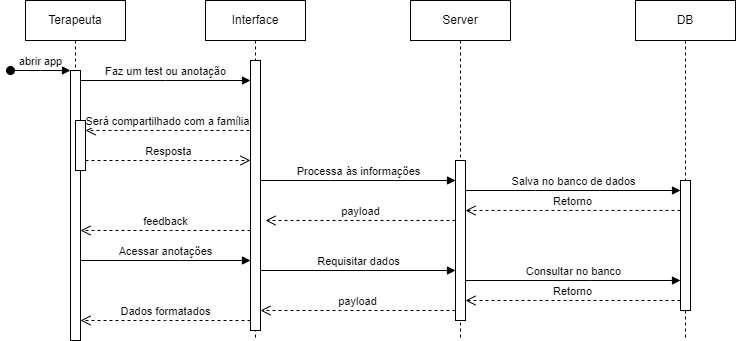
\includegraphics[scale=0.5]{imagens/Diagrama do terapeuta.drawio.png} \\
    \label{fig:digrama_sequencia_terapeuta}
    {
        Fonte: Elaborado pelo autor
    }
\end{figure}

O perfil de família só pode ter acesso ao paciente ao qual está relacionado, 
permitindo-lhe acessar apenas os dados autorizados pelo terapeuta. 
A família deve ter a capacidade de fazer anotações. Sempre que a família acessar a sessão de anotações, 
o \textit{software} deve realizar uma requisição para verificar se as anotações estão atualmente permitidas pelo terapeuta. 
O fluxo desse funcionamento pode ser visualizado na Figura~\ref{fig:digrama_sequencia_familia}.

\begin{figure}[!htb]
{}
    \centering
    \caption{Diagrama de sequência com perfil de família detalhando as principais ações da família na utilização do sistema}
    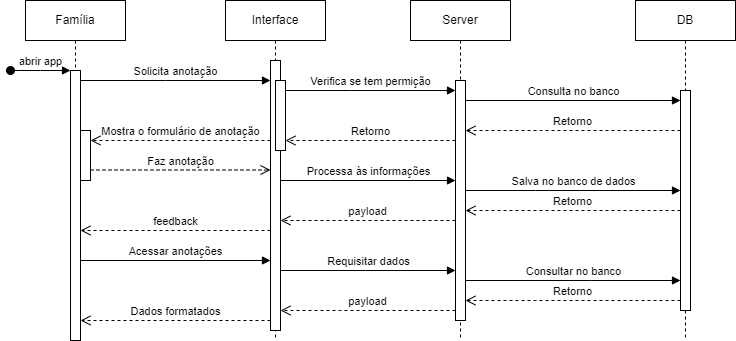
\includegraphics[scale=0.5]{imagens/Diagrama do Usuário.drawio.png} \\
    \label{fig:digrama_sequencia_familia}
    {
        Fonte: Elaborado pelo autor
    }
\end{figure}

Ambos os perfis de usuários têm a opção de desvincular um paciente de um terapeuta ou da rede de terapeutas. 
No caso de desvinculação, a família terá acesso a todas as anotações relacionadas ao paciente, 
enquanto o terapeuta não terá mais acesso a essas anotações. No entanto, 
os dados continuarão a ser utilizados para gerar estatísticas exibidas na página principal. 
Essas diretrizes estarão claramente detalhadas nos termos de serviço e serão apresentadas antes de qualquer solicitação 
de desvinculação.

As anotações têm como principal objetivo auxiliar o método ABA nos levantamentos de dados. 
Embora o \textit{software} tenha alguns recursos voltados para a técnica do ABA treino por tentativas discretas, 
foi projetado para permitir anotações variadas relevantes para profissionais que trabalham com pacientes e suas famílias.

\section{Experiencia do Usuário}

Com a finalidade de proporcionar uma melhor interatividade, 
é essencial compreender as necessidades do público-alvo. 
om esse propósito, foram criadas duas personas (personagens fictícios representando usuários típicos) 
para ilustrar as expectativas e comportamentos do grupo de usuários. 
Essas personas são detalhadas nas Figuras \ref{fig:persona_joao} e \ref{fig:persona_maria}.

\begin{figure}[!htb]
{}
    \caption{Persona elaborada para representar um usuário com maior familiaridade no uso de \textit{softwares}.}
    \centering
    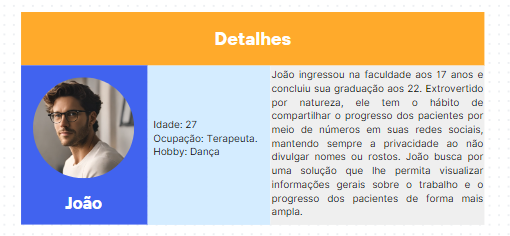
\includegraphics[scale=1.0]{imagens/Joao.png} \\
    \label{fig:persona_joao}
    {
        Fonte: Elaborado pelo autor
    }
\end{figure}

\begin{figure}[!htb]
{}
    \caption{
        Persona elaborada para representar um usuário com menor familiaridade no uso de \textit{software}, 
        necessitando de uma experiência mais intuitiva.
    }
    \centering
    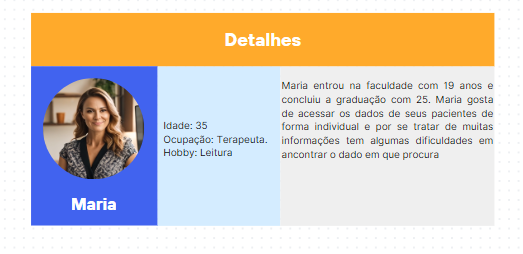
\includegraphics[scale=1.0]{imagens/Maria.png} \\
    \label{fig:persona_maria}
    {
        Fonte: Elaborado pelo autor
    }
\end{figure}

Com a análise das personas, é possível obter uma compreensão mais aprofundada sobre o desenvolvimento da aplicação. 
Considerando que o público-alvo possa ser composto por indivíduos com pouca experiência em aplicativos, 
é fundamental que o design seja intuitivo e acessível a uma ampla gama de usuários. 
Portanto, o \textit{software} deve fornecer informações claras e explicativas sobre as funcionalidades de cada seção.

Em várias áreas do \textit{software}, é crucial oferecer uma indicação clara da seção atual, 
do caminho percorrido pelo usuário e das possíveis direções futuras, 
como demonstrado no fluxo de navegação apresentado na Figura \ref{fig:fluxo_de_navegacao}. 
Cada conjunto de dados deve ser acompanhado por uma breve descrição, 
priorizando a simplicidade para evitar a sobrecarga de informações em espaços limitados, 
o que poderia gerar confusão ao usuário.

\begin{figure}[phtb]
{}
    \caption{Fluxo de navegação}
    \centering
     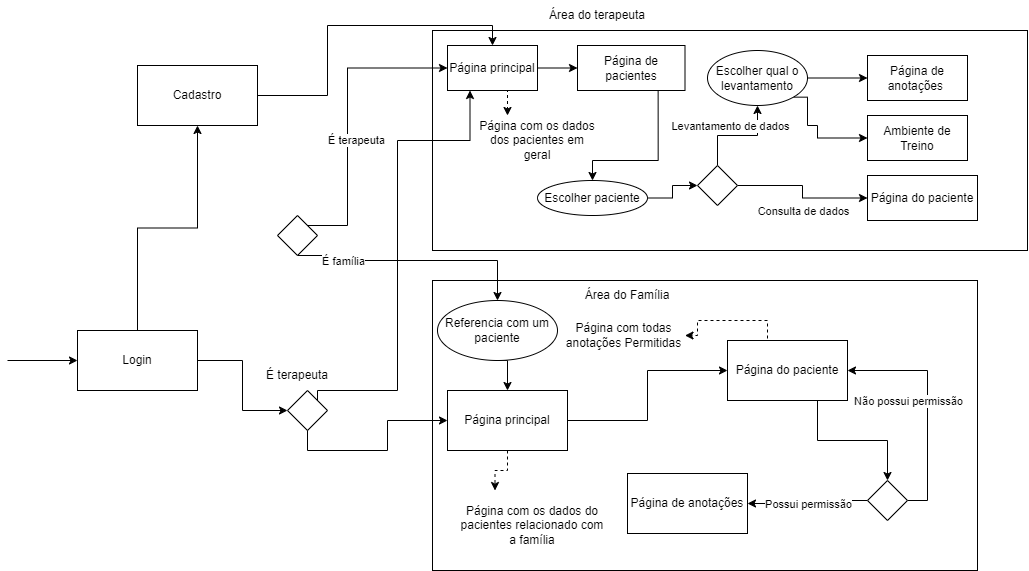
\includegraphics[scale=0.4]{imagens/Fluxo de navegação.png} \\
    \label{fig:fluxo_de_navegacao}
    {
        Fonte: Elaborado pelo autor
    }
\end{figure}

Considerando que o \textit{software} é destinado a terapeutas e familiares de pacientes, 
é crucial proporcionar aos usuários uma sensação de seriedade e confiança durante sua utilização profissional. 
Por essa razão, o \textit{software} foi desenvolvido com tonalidades que variam entre azul escuro e ciano, 
cores conhecidas por transmitirem seriedade e tranquilidade. 
No entanto, ao lidar com os exercícios para os pacientes, que requerem maior interação, 
o uso de cores opostas no círculo cromático, como verde e tons sutis de roxo, 
visa atrair a atenção das crianças e proporcionar uma atmosfera mais alegre.

\subsection{Procedimentos de Validação de Usabilidade}\label{subsec:validacao_usabilidade}

Para validar a usabilidade do \textit{software}, serão conduzidos testes com profissionais da área. 
Esses testes serão realizados em ambiente controlado, 
no qual os participantes serão convidados a executar tarefas específicas utilizando o sistema.

Os testes serão divididos em duas etapas: a primeira permitirá o uso do sistema durante a sessão terapêutica,
enquanto a segunda consistirá na realização da terapia sem a utilização do \textit{software}. Em ambas as etapas, 
serão coletados dados referentes à experiência dos usuários, incluindo \textit{feedback} qualitativo e quantitativo. 
A análise desses dados possibilitará avaliar a eficácia do \textit{software} na melhoria da experiência terapêutica, 
bem como identificar aspectos passíveis de aperfeiçoamento.

Os dados coletados pelos terapeutas não serão utilizados para fins clínicos ou de pesquisa sobre pacientes, 
mas exclusivamente para avaliação da usabilidade do sistema e identificação de possíveis melhorias. 
O \textit{feedback} fornecido pelos profissionais será fundamental para o aprimoramento da interface e das funcionalidades, 
garantindo que o \textit{software} atenda de forma adequada às necessidades dos usuários, 
além de possibilitar a análise de sua viabilidade como ferramenta de apoio à aplicação do método ABA, 
considerando a experiência dos terapeutas e a interação com familiares dos pacientes.

Na etapa sem utilização do \textit{software}, os terapeutas realizarão registros por meio de métodos tradicionais, 
utilizando papel e caneta. Posteriormente, essas anotações serão comparadas às realizadas no sistema, 
com o objetivo de analisar a eficiência e a facilidade de uso da ferramenta em relação às práticas convencionais.

Além disso, os testes contarão com a participação de aproximadamente 10 profissionais da área, 
selecionados por conveniência, considerando sua experiência prévia com intervenções baseadas no método ABA. 
Como instrumentos de coleta de dados, serão utilizados questionários estruturados com escala do tipo Likert para 
avaliação quantitativa da usabilidade, bem como formulários abertos para obtenção de \textit{feedback} qualitativo. 
Também poderão ser registrados o tempo de execução das tarefas e a ocorrência de dificuldades operacionais durante 
o uso do sistema.  Para a análise dos dados, será realizada uma abordagem mista: 
os dados quantitativos serão tratados por meio de estatística descritiva (média, desvio padrão e frequência de respostas), 
enquanto os dados qualitativos serão analisados por categorização temática, permitindo a identificação de padrões, 
percepções recorrentes e oportunidades de melhoria no sistema.

Cabe ressaltar que, por questões éticas e de privacidade relacionadas aos dados dos pacientes,
os pesquisadores não terão acesso direto às anotações clínicas realizadas durante as sessões terapêuticas. 
Dessa forma, métricas como o tempo necessário para realização das anotações
ou a quantidade de informações registradas não serão coletadas diretamente pelo sistema.

Essas informações poderão ser relatadas pelos próprios terapeutas por meio dos formulários
de avaliação aplicados após a utilização do sistema. Assim, os participantes poderão informar,
de forma aproximada, sua percepção sobre o tempo gasto nas anotações e a quantidade de dados
registrados, tanto utilizando o \textit{software} quanto por meio dos métodos tradicionais.
Essa abordagem busca preservar a confidencialidade dos dados dos pacientes, ao mesmo tempo
em que possibilita obter percepções relevantes sobre a eficiência e a usabilidade da ferramenta.

\subsection{Instrumentos de coleta de dados}
Para avaliação da usabilidade do sistema, foi utilizado um questionário estruturado
com escala Likert de cinco pontos.

As perguntas aplicadas aos participantes incluíram:

\begin{itemize}
\item O sistema foi fácil de aprender a utilizar.
\item A interface é clara e intuitiva.
\item O sistema facilitou o registro das informações durante a terapia.
\item O sistema contribui para melhorar a organização dos dados.
\item Eu utilizaria o sistema em minha prática profissional.
\end{itemize}

Além das questões de usabilidade, o formulário também incluiu perguntas voltadas à
percepção dos profissionais sobre o processo de registro das informações durante
as sessões terapêuticas. Entre essas questões, destacam-se:

\begin{itemize}
\item Durante a sessão com a utilização do \textit{software} quanto tempo durou a sessão?
\item Durante a sessão com a utilização do \textit{software} quantas anotações foram feitas?
\item Durante a sessão sem a utilização do \textit{software} quanto tempo durou a sessão?
\item Durante a sessão sem a utilização do \textit{software} quantas anotações foram feitas?
\end{itemize}

% \section{Interface do Usuário}
\section{Interface do Usuário}\label{sec:interface_usuário}

Esta seção se concentra na análise minuciosa dos componentes e na interação do usuário com a interface. 
Explora-se a experiência do usuário ao utilizar o sistema e sua interação com os diversos elementos da interface. 
O objetivo é permitir a concentração na estrutura e na disposição dos elementos visuais, 
possibilitando uma compreensão mais rápida e uma avaliação direta do \textit{layout} e das interações.

No processo de \textit{login}, são inseridas as credenciais, 
concedendo diferentes níveis de acesso no sistema. 
A seção destinada às famílias permite acesso apenas às anotações autorizadas pelo terapeuta referentes 
ao paciente específico, além de permitir fazer anotações, quando autorizado pelo terapeuta. 
A tela de login possui uma rota para o cadastro, 
onde o usuário deve especificar o tipo de acesso desejado. No caso de acesso como família, 
é necessário vincular-se a um paciente previamente cadastrado por um terapeuta. 
Como apresentada na figura \ref{fig:login} e na figura \ref{fig:register}.

\begin{figure}[p]
{}
    \begin{minipage}[b]{0.5\linewidth}
        \caption{Página de \textit{login}}
        \centering
        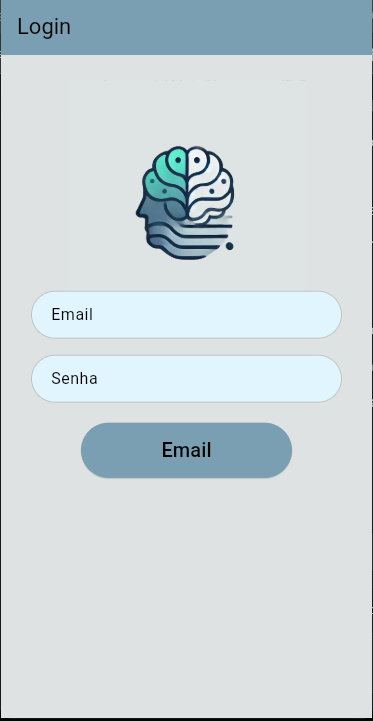
\includegraphics[scale=0.27]{imagens/LoginPage.png} \\
        \label{fig:login}
        {
            Fonte: Elaborado pelo autor
        }
    \end{minipage}
    \begin{minipage}[b]{0.5\linewidth}
        \caption{Página de cadastro}
        \centering
        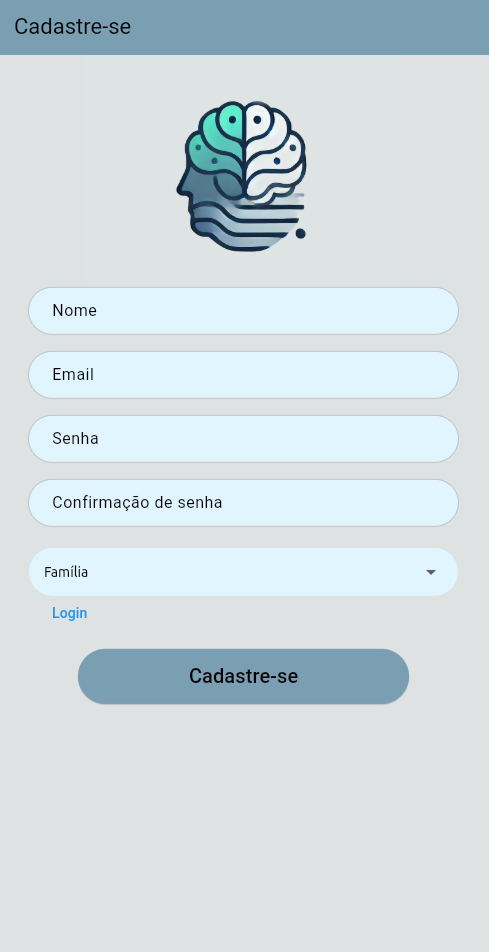
\includegraphics[scale=0.36]{imagens/RegisterPage.png} \\
        \label{fig:register}
        {
            Fonte: Elaborado pelo autor
        }
    \end{minipage}
\end{figure}

Na página principal, um gráfico exibirá os dados sobre o número de pacientes em cada nível 
de dificuldade dos treinos. Os níveis serão representados por barras, 
cada uma identificada por uma \textit{label} e um número acima, indicando a quantidade 
correspondente de pacientes. Como apresentado na figura \ref{fig:home}.

\begin{figure}[p]
{}
    \caption{Página principal}
    \centering
    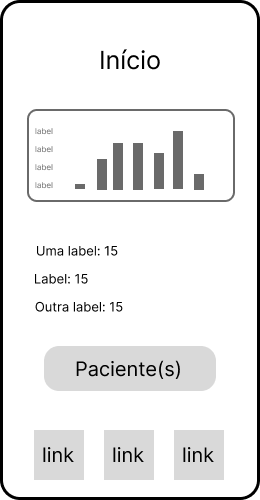
\includegraphics[scale=0.5]{imagens/HomePage.png} \\
    \label{fig:home}
    {
        Fonte: Elaborado pelo autor
    }
\end{figure}  


Botões de tamanho ampliado visam aumentar a acessibilidade, acompanhados por descrições 
ou ícones indicativos das seções correspondentes, constituindo a principal forma de navegação 
no aplicativo. Adicionalmente, um componente exibe as três últimas telas da pilha de navegação, 
permitindo visualizar a tela atual e as duas anteriores.

No cenário do usuário estar logado com o perfil de família, ele não pode ter acesso à lista de 
pacientes e, no lugar disso, ele vai direto à parte do perfil do paciente. Caso o usuário acesse 
com o perfil de terapeuta, ele precisa acessar uma lista de pacientes e precisa selecionar um 
paciente para ter acesso às anotações feitas para aquele paciente.

No cabeçalho da tela, há um texto indicativo sobre como acessar a página do paciente e iniciar 
o levantamento de dados. Ao tentar acessar a página de levantamento de dados, o terapeuta encontra 
um modal solicitando a seleção do tipo de levantamento desejado. Como demonstrado na figura 
\ref{fig:patients_page} e \ref{fig:patients_modal}. 

\begin{figure}[h]
{}
    \begin{minipage}[b]{0.5\linewidth}
        \caption{Página de pacientes, exibindo uma lista de todos os pacientes}
        \centering
        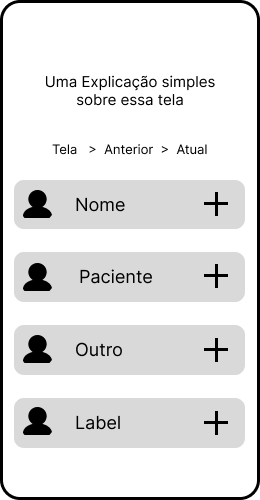
\includegraphics[scale=0.35]{imagens/PatientsPage.png} \\
        \label{fig:patients_page}
        {
            Fonte: Elaborado pelo autor
        }
    \end{minipage}
    \begin{minipage}[b]{0.5\linewidth}
        \caption{Modal de anotações}
        \centering
        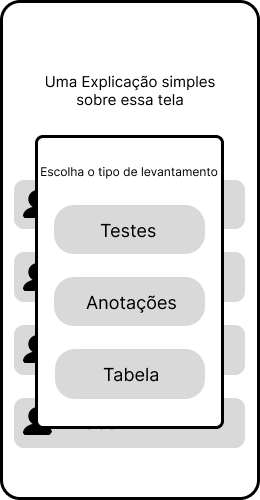
\includegraphics[scale=0.35]{imagens/PatientsModal.png} \\
        \label{fig:patients_modal}
        {
            Fonte: Elaborado pelo autor
        }
    \end{minipage}
\end{figure}

No cabeçalho da tela de perfil do paciente, são exibidos alguns dados do paciente, 
enquanto no corpo da tela são apresentados \textit{cards} contendo informações sobre 
as anotações ou tabelas (anotadas ou geradas na área de treinos). Ao tocar nesses 
\textit{cards}, eles se expandem, exibindo todo o conteúdo, como demonstrado na Figura 
\ref{fig:patient_detail} e na Figura \ref{fig:patient_detail_expanded}. Além disso, na mesma tela, 
é exibido um \textit{card} que, ao ser tocado, apresenta algumas opções de filtro, 
conforme ilustrado na Figura \ref{fig:patient_expanded_filter}.

\begin{figure}[hb]
{}
    \begin{minipage}[b]{0.5\linewidth}
        \caption{Página de perfil listando todas anotações disponíveis}
        \centering
        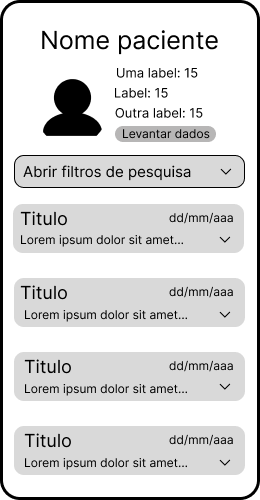
\includegraphics[scale=0.35]{imagens/PatientDetail.png}\\
        \label{fig:patient_detail}
        {
            Fonte: Elaborado pelo autor
        }
    \end{minipage}
    \begin{minipage}[b]{0.5\linewidth}
        \caption{Perfil com anotação expandida}
        \centering
        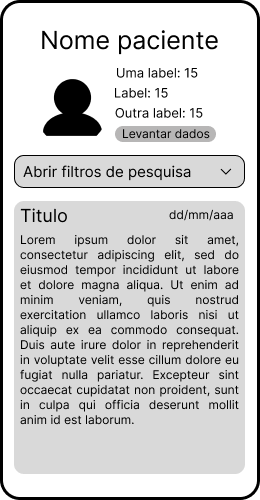
\includegraphics[scale=0.35]{imagens/PatientDetailExpanded.png} \\
        \label{fig:patient_detail_expanded}
        {
            Fonte: Elaborado pelo autor
        }
    \end{minipage}
\end{figure}

\begin{figure}[!b]
{}
    \caption{Página de pacientes com filtro estendido}
    \centering
    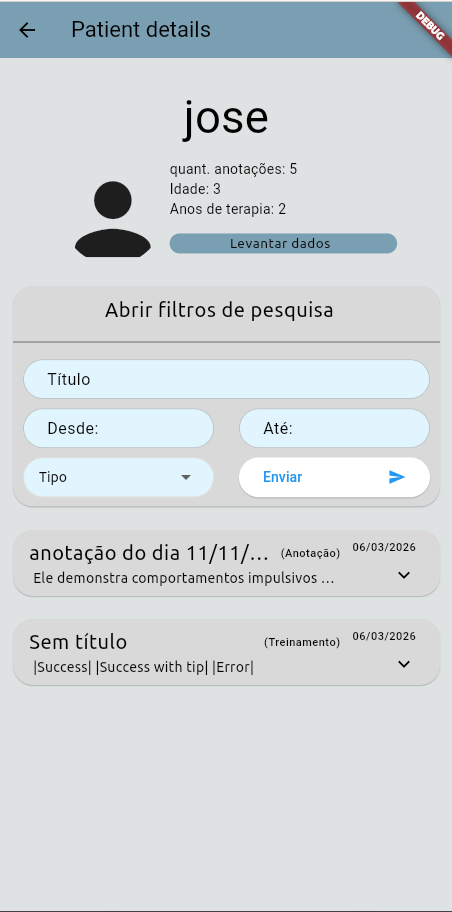
\includegraphics[scale=0.35]{imagens/PatientFilter.png} \\
    \label{fig:patient_expanded_filter}
    {
        Fonte: Elaborado pelo autor
    }
\end{figure}  

Quanto às formas de anotação, há dois tipos principais: uma semelhante a um bloco de notas 
e outra em formato de tabela. Na opção de tabela, o terapeuta pode pré-selecionar várias 
opções para inserir dados, permitindo adicionar, remover ou editar conforme necessário.

\begin{figure}[!htb]
{}
    \caption{Anotação por tabela}
    \centering
    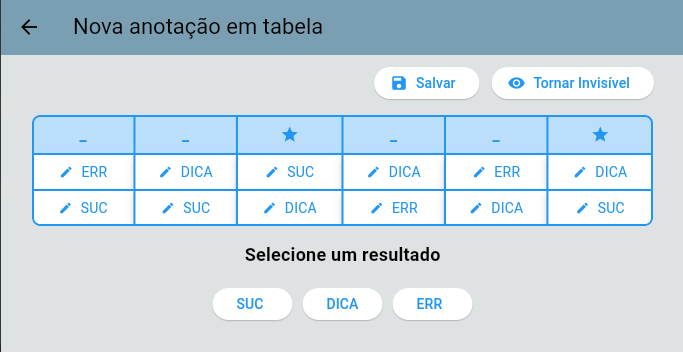
\includegraphics[scale=0.7]{imagens/Table.png} \\
    \label{fig:anotacao_table}
    {
        Fonte: Elaborado pelo autor
    }
\end{figure}

\begin{figure}[!htb]
{}
    \caption{Anotação por texto}
    \centering
    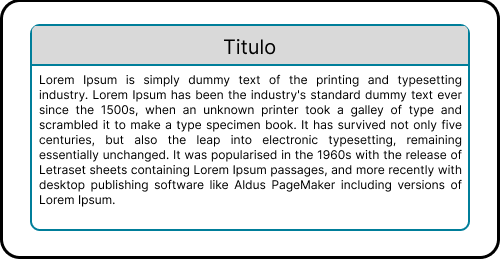
\includegraphics[scale=0.7]{imagens/TextEditor.png} \\
    \label{fig:anotacao_text}
\end{figure}

Há também uma área de treinos voltada para o Treino por Tentativas Discretas, 
assemelhando-se a um jogo, onde o paciente interage tocando em cartões na tela. 
Quando bem-sucedido, o paciente recebe um reforço. Dependendo da configuração 
prévia realizada pelo terapeuta, o aplicativo pode incluir animações para o paciente. 
Os dados gerados a partir das anotações ou dos treinos são armazenados e podem ser 
posteriormente consultados.

Os cartões devem ter cores chamativas e conter uma imagem central. No cenário de sucesso, 
não é estritamente necessário tocar precisamente no cartão; também é possível interagir 
em uma área ao redor dele para uma melhor acessibilidade (a área é determinada pelo terapeuta). 
Cada programa de treino oferece uma interação diferente com o paciente, e cada nível de dificuldade 
tem respostas distintas às interações do paciente.

No programa por correspondência, é apresentado um cartão para o paciente e uma quantidade 
$n$ de cartões para o paciente. O terapeuta emite o comando (algo como: "Corresponda"), 
e o cenário de sucesso é tocar no cartão ou próximo a ele, referente àquele cartão mostrado 
para o paciente (a posição do cartão pode ser configurada em cima, direita, embaixo ou esquerda, 
dependendo da configuração escolhida pelo terapeuta).
% O protótipo da tela do treino pode ser visto na Figura \ref{fig:mathing}.


\begin{figure}[!hb]
{}
    \caption{Treino por correspondência onde o sucesso é interagir com o cartão que corresponde à imagem}
    \centering
    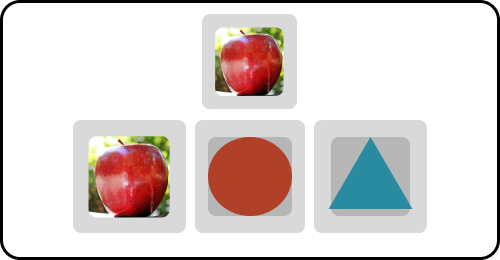
\includegraphics[scale=0.6]{imagens/TrainingMathing.png} \\
    \label{fig:mathing}
    {
        Fonte: Elaborado pelo autor
    }
\end{figure}

No programa receptivo, são apresentados uma quantidade $n$ de cartões, 
e o terapeuta emite o comando (algo como: "toque no 'item'"). O cenário de 
sucesso é tocar no cartão ou próximo a ele, referente àquele item mencionado. 
O protótipo da tela do treino pode ser visto na Figura \ref{fig:receptive}.


\begin{figure}[!hb]
{}
    \caption{Treino receptivo onde o sucesso é interagir com o cartão referente ao comando do terapeuta}
    \centering
    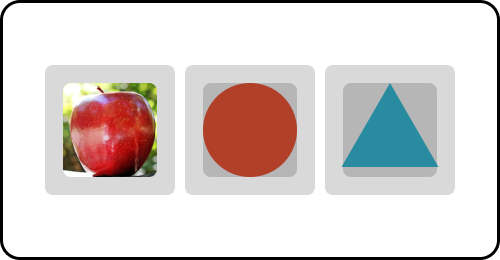
\includegraphics[scale=0.6]{imagens/TrainingReceptive.png} \\
    \label{fig:receptive}
    {
        Fonte: Elaborado pelo autor
    }
\end{figure}

No programa expressivo, é mostrado um único cartão para o paciente 
(o comando pode ser algo como: "o que é isso?" ou "qual o nome disso?"). 
Para contar como cenário de sucesso, o terapeuta deve tocar no botão de sucesso. 
Nesse cenário, o terapeuta valida o sucesso da criança, já que no programa expressivo, 
o paciente deve falar o nome do item para obter sucesso. O protótipo da tela do treino 
pode ser visto na Figura \ref{fig:exprecive}.

\begin{figure}[!htb]
{}
    \caption{Treino expressivo onde o sucesso é o terapeuta tocar no botão de sucesso}
    \centering
    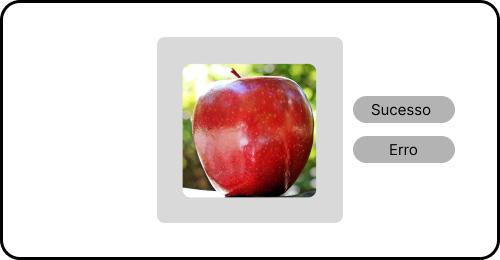
\includegraphics[scale=0.6]{imagens/TrainingExprecive.png} \\
    \label{fig:exprecive}
    {
        Fonte: Elaborado pelo autor
    }
\end{figure}


